	\section{Anexos}
	
	\subsection{Análisis exploratorio del conjunto de datos}
	
	El análisis exploratorio de datos (EDA, por sus siglas en inglés) es una etapa fundamental dentro del desarrollo de sistemas basados en aprendizaje automático y visión por computadora, debido a que permite comprender la estructura, distribución y comportamiento de las muestras antes del entrenamiento de los modelos \cite{tukey1977eda,geron2022hands}. 
	
	De acuerdo con Tukey \cite{tukey1977eda}, esta fase facilita la identificación de patrones, anomalías, dispersiones y características relevantes dentro de un conjunto de datos, optimizando la toma de decisiones durante el diseño estructural del sistema. La importancia de este análisis a que la calidad, diversidad y representación de los datos de entrada influyen directamente en la capacidad de generalización y robustez final de los clasificadores \cite{goodfellow2016deep}.
	
	En el presente trabajo la exploración se centrará en el estudio de la representación geométrica de las señas mediante los puntos de referencia (\textit{landmarks}) extraídos con MediaPipe Hands, evaluando la distribución y variabilidad del conjunto de datos construido para el reconocimiento de señas estáticas de la LSM. A diferencia de los enfoques tradicionales basados en procesamiento directo de imágenes RGB, la abstracción mediante un vector reduce  la complejidad computacional y el ruido de entrada al conservar exclusivamente la información espacial y dimensional asociada a la morfología de la mano \cite{mediapipe_hands}.
	
	A través de los siguientes apartados se evalúa la distribución de las clases, la variabilidad espacial provocada por las condiciones de captura y la separabilidad del espacio de características. Este análisis permitirá justificar los criterios de diseño para el pipeline de preprocesamiento local, la ingeniería de características y la selección de las arquitecturas de clasificación que se desarrollarán en este proyecto.
	
	\subsubsection{Descripción general del conjunto de datos}
	
	
	Debido a la limitada disponibilidad de repositorios públicos orientados a la LSM que sean compatibles con enfoques basados en \textit{landmarks}, se optó por la creación de un conjunto de datos propio.
	
	El dataset final quedó conformado por un total de 159650 muestras vectoriales válidas, distribuidas en 21 clases distintas que corresponden a las configuraciones estáticas del alfabeto manual. Las clases consideradas para este desarrollo fueron: A, B, C, D, E, F, G, H, I, L, M, N, O, P, R, S, T, U, V, W y Y.
	
	Con la finalidad de incrementar la robustez de los modelos ante variaciones en la orientación de la mano, se aplicaron técnicas de aumento de datos mediante transformaciones horizontales (\textit{flip}) directamente sobre las coordenadas de los puntos extraídos. Esto permitió duplicar la cantidad de muestras simulando el uso de la mano contraria, ampliando la variabilidad del conjunto de datos sin alterar la forma ni el significado de las señas.
	
	Cabe destacar que aquellas letras que requieren estrictamente de un componente dinámico, movimiento o traslación temporal para su interpretación (tales como la "J", "K", "Ñ", "Q", "X" y "Z") fueron excluidas. Esta delimitación responde directamente al alcance del presente trabajo, el cual se enfoca exclusivamente en el reconocimiento robusto de configuraciones estáticas de la mano.
	
	La Tabla \ref{tab:dataset_general} presenta la distribución general de las muestras válidas por cada clase dentro del conjunto de datos final que será utilizado para los experimentos de entrenamiento y evaluación de los modelos clasificadores.
	
	\begin{table}[H]
		\centering
		
		\rowcolors{2}{rowblue}{white}
		
		\caption{Distribución de muestras por clase del conjunto de datos final}
		\label{tab:dataset_general}
		
		\small
		\renewcommand{\arraystretch}{1.2}
		
		\begin{tabular}{|p{3cm}|p{4cm}|}
			\hline
			
			\rowcolor{headerblue}
			\headercell{Clase} &
			\headercell{Número de muestras} \\
			\hline
			
			A & 7567 \\
			B & 7771 \\
			C & 7800 \\
			D & 7714 \\
			E & 7432 \\
			F & 7690 \\
			G & 7748 \\
			H & 7800 \\
			I & 7383 \\
			L & 7602 \\
			M & 7467 \\
			N & 7392 \\
			O & 7800 \\
			P & 7749 \\
			R & 7521 \\
			S & 7249 \\
			T & 7703 \\
			U & 7336 \\
			V & 7520 \\
			W & 7606 \\
			Y & 7800 \\
			\hline
			
			\rowcolor{headerblue}
			\textbf{Total} & \textbf{159650} \\
			\hline
			
		\end{tabular}
		
	\end{table}
	
	
	\subsubsection{Análisis de distribución de clases}
	
	El balance en la cantidad de muestras por cada clase es un factor crítico en el entrenamiento de modelos de clasificación. Un desbalance considerable provocaría que el modelo se incline por las clases mayoritarias, afectando su precisión general \cite{goodfellow2016deep}. Por ello el diagnóstico inicial del conjunto de datos se enfoca en evaluar la simetría en la frecuencia de las señas capturadas.
	
	La Figura \ref{fig:distribucion_dataset} (que complementa los datos del Cuadro \ref{tab:dataset_general}) muestra la distribución final de las muestras válidas para cada una de las 21 clases del alfabeto de la LSM considerado.
	
	\begin{figure}[H]
		\centering
		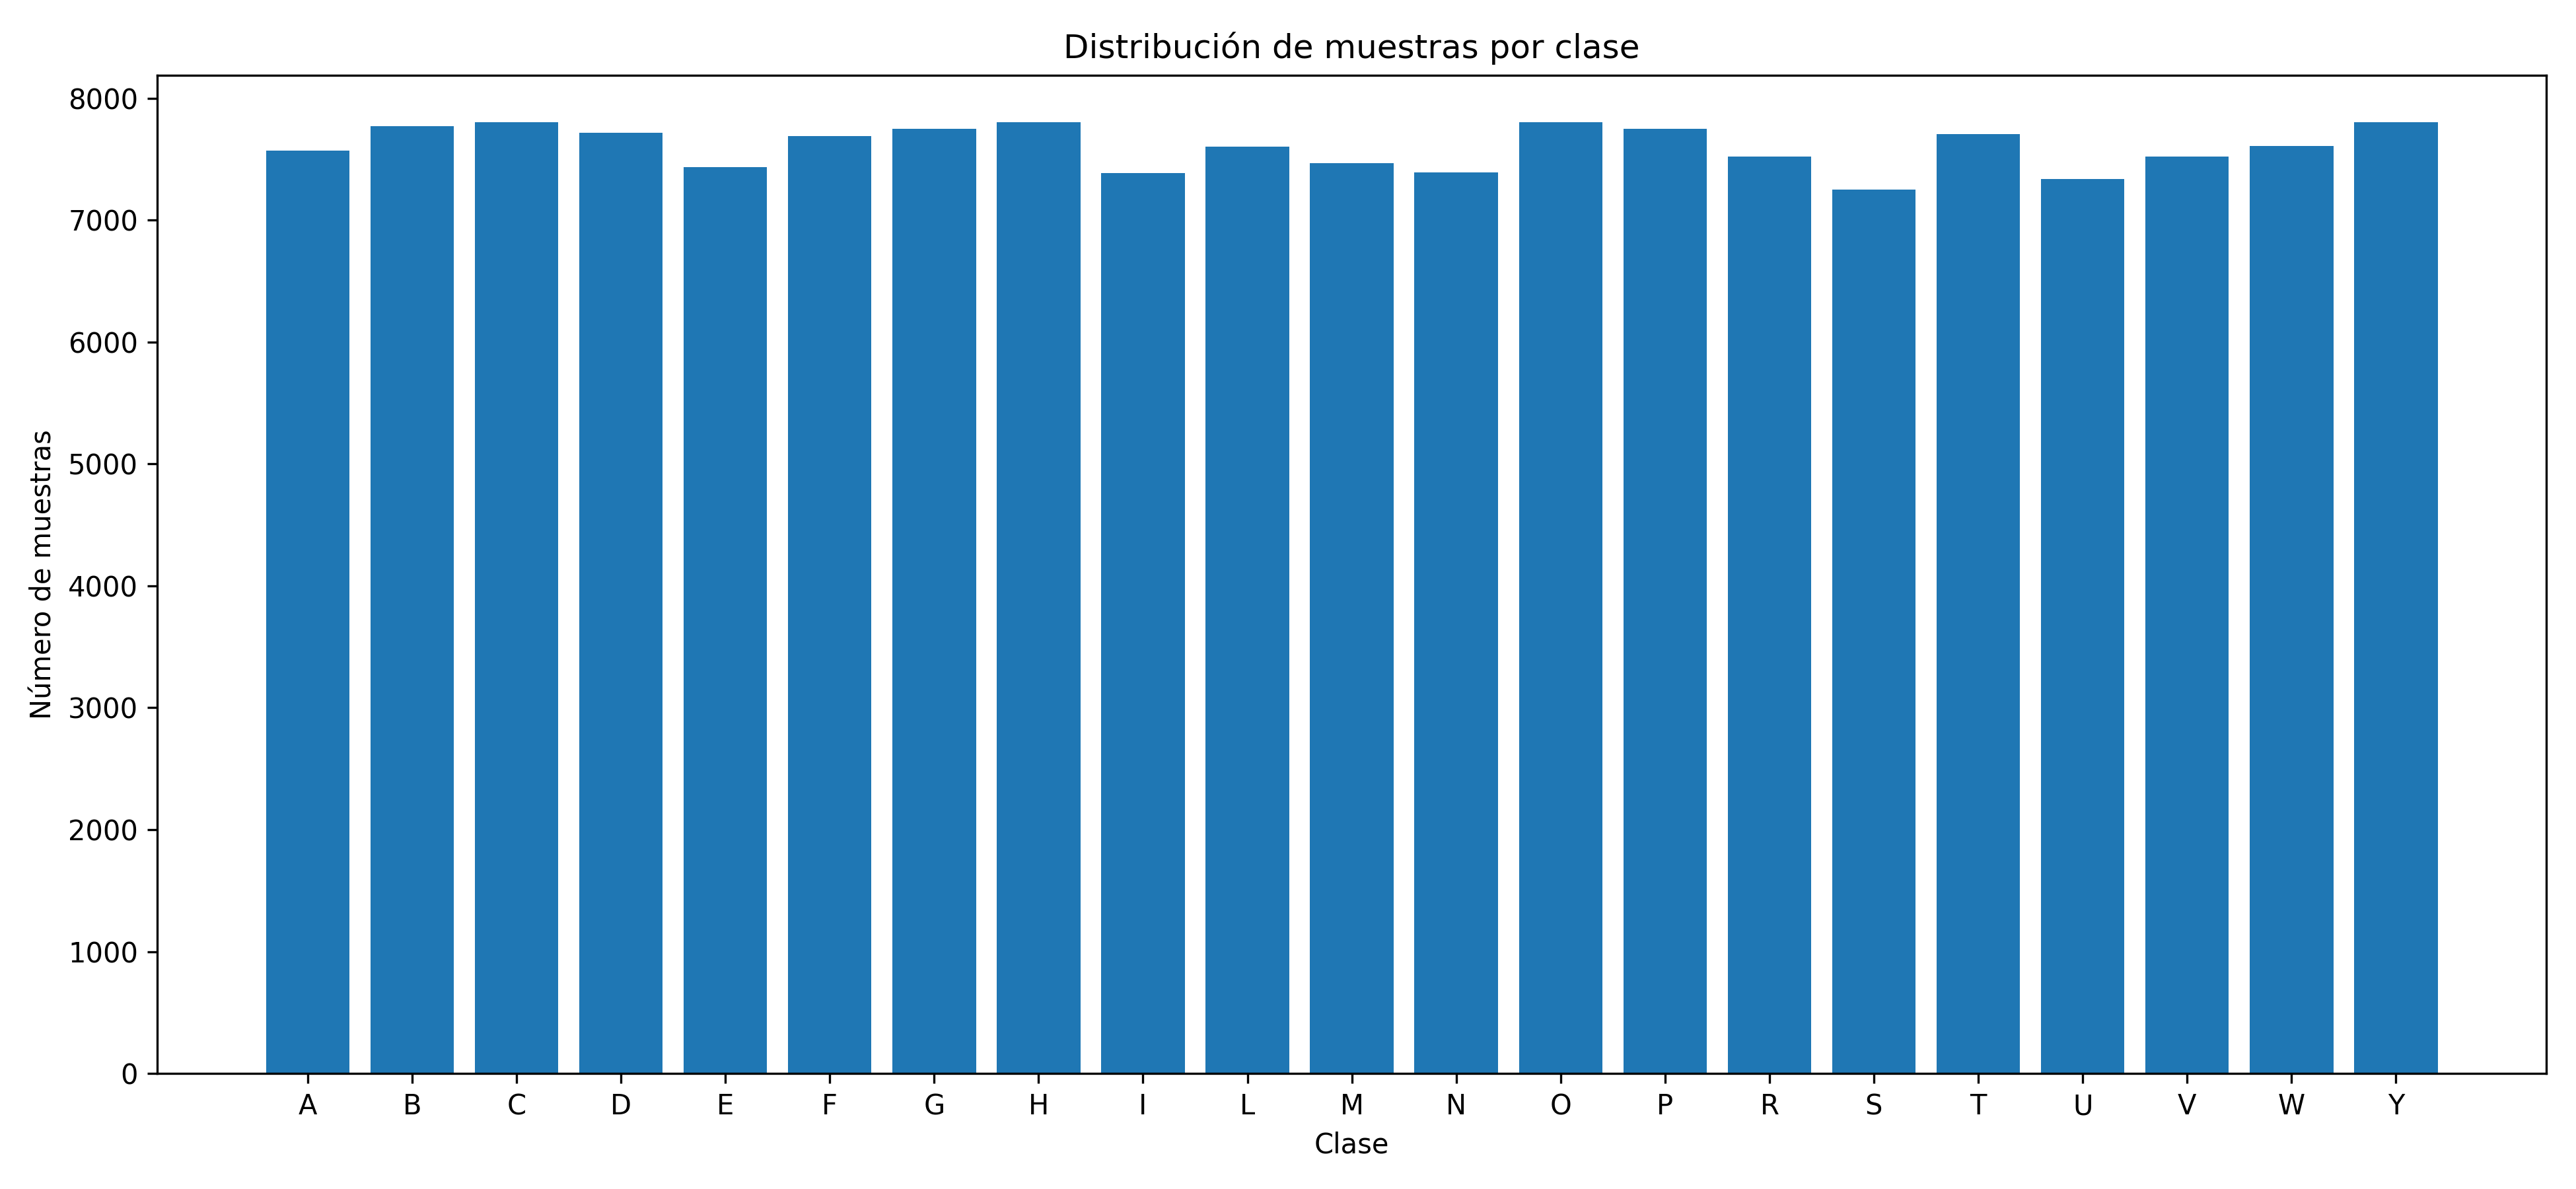
\includegraphics[width=0.95\textwidth]{images/distribucion_clases.png}
		\caption{Distribución de muestras por clase del conjunto de datos final}
		\label{fig:distribucion_dataset}
	\end{figure}
	
	Como se observa en la Figura \ref{fig:distribucion_dataset}, el conjunto de datos presenta una distribución relativamente homogénea entre las clases, manteniéndose la mayoría de ellas en un rango aproximado entre 7200 y 7800 muestras. Esta distribución equilibrada es un indicador positivo preliminar, ya que teóricamente reduce el riesgo de sesgo hacia clases mayoritarias durante la posterior etapa de entrenamiento.
	
	Desde la perspectiva del diseño del sistema, este balance uniforme permite proyectar el uso de funciones de pérdida estándar para la clasificación multiclase, tales como la entropía cruzada categórica (\textit{Categorical Cross-Entropy}) o su variante dispersa (\textit{Sparse Categorical Cross-Entropy}), las cuales basan su eficacia en la suposición de clases equitativas durante el cálculo del gradiente \cite{goodfellow2016deep}. Por otro lado la paridad en los conteos preliminares sugiere que, en principio, es viable prescindir de técnicas complejas de sobremuestreo artificial o de la implementación de funciones de pérdida modificadas, estrategias comúnmente requeridas para mitigar el sesgo en distribuciones asimétricas dentro de tareas modernas de visión artificial \cite{johnson2021survey, fujiwara2025class}.
	
	\subsubsection{Análisis de variabilidad geométrica y espacial}
	
	A diferencia de un análisis basado en imágenes completas, revisar la variación de los puntos de la mano requiere entender cómo cambian los números de las coordenadas dentro del lienzo de captura. Al revisar los datos del DataFrame, se observa que las coordenadas entregadas por MediaPipe ya vienen normalizadas en un rango de 0 a 1 respecto al ancho y alto de la pantalla. Sin embargo, este ajuste inicial no funciona para nuestro objetivo, ya que a nosotros no nos interesa saber la distancia ni en qué lugar de la imagen se encuentra la mano, sino conocer su configuración geométrica pura.
	
	En primer lugar, revisamos cómo cambia el tamaño de la mano en la pantalla debido a la distancia de captura. La Figura \ref{fig:histograma_escala} muestra la distribución obtenida al calcular la distancia entre la muñeca (\textit{landmark} 0) y la base del dedo medio (\textit{landmark} 9) para todo el conjunto de datos crudos.
	
	\begin{figure}[H]
		\centering
		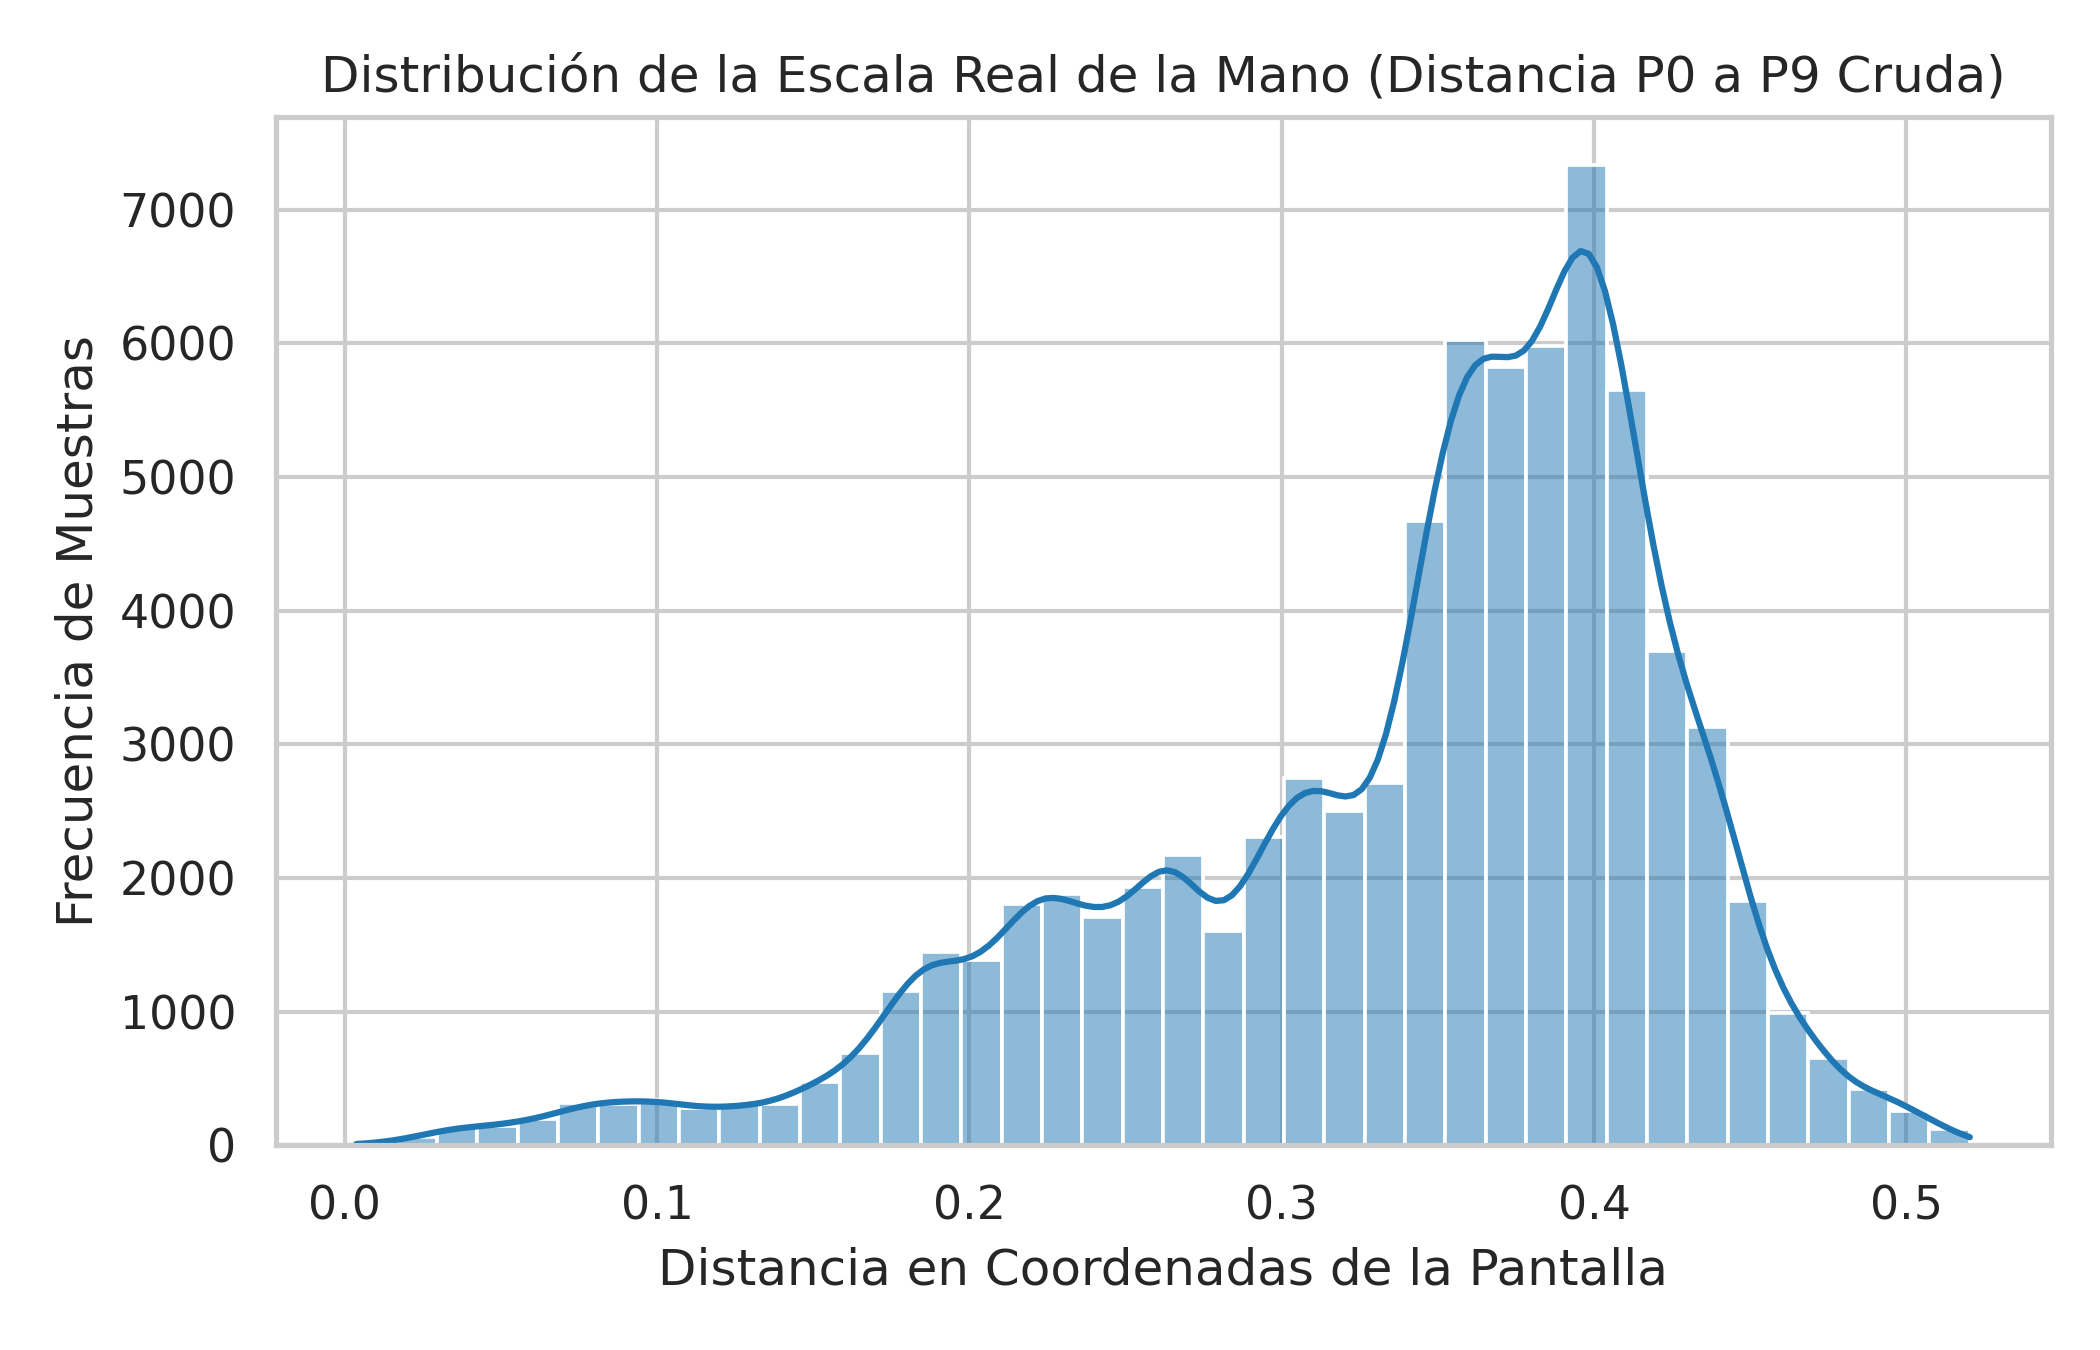
\includegraphics[width=0.90\textwidth]{images/nuevo_histograma_escala.png}
		\caption{Distribución del tamaño relativo de la palma en los datos crudos}
		\label{fig:histograma_escala}
	\end{figure}
	
	Como se ve en la Figura \ref{fig:histograma_escala}, las distancias se encuentran distribuidas entre menos de 0.1 y un máximo cercano a 0.52, concentrando la mayor parte de las muestras entre 0.35 y 0.42. Esta dispersión confirma que, aunque MediaPipe acote los valores al tamaño de la pantalla, el tamaño relativo de la mano cambia notablemente según qué tan lejos se coloque cada usuario. Si se intentara entrenar un modelo con estos datos de forma directa, el sistema podría confundir el tamaño o el encuadre con la identidad de la seña, lo que justifica la necesidad de buscar un método propio para aislar la forma de la mano independientemente de su escala.
	
	
	En segundo lugar, se utilizan diagramas de boxplot para evaluar la dispersión de las posiciones de los dedos en una misma seña tomando los datos crudos. La Figura \ref{fig:boxplot_variabilidad} muestra las distancias calculadas desde la muñeca hasta las puntas de los cinco dedos, utilizando las muestras de la letra A como escenario de prueba.
	
	\begin{figure}[H]
		\centering
		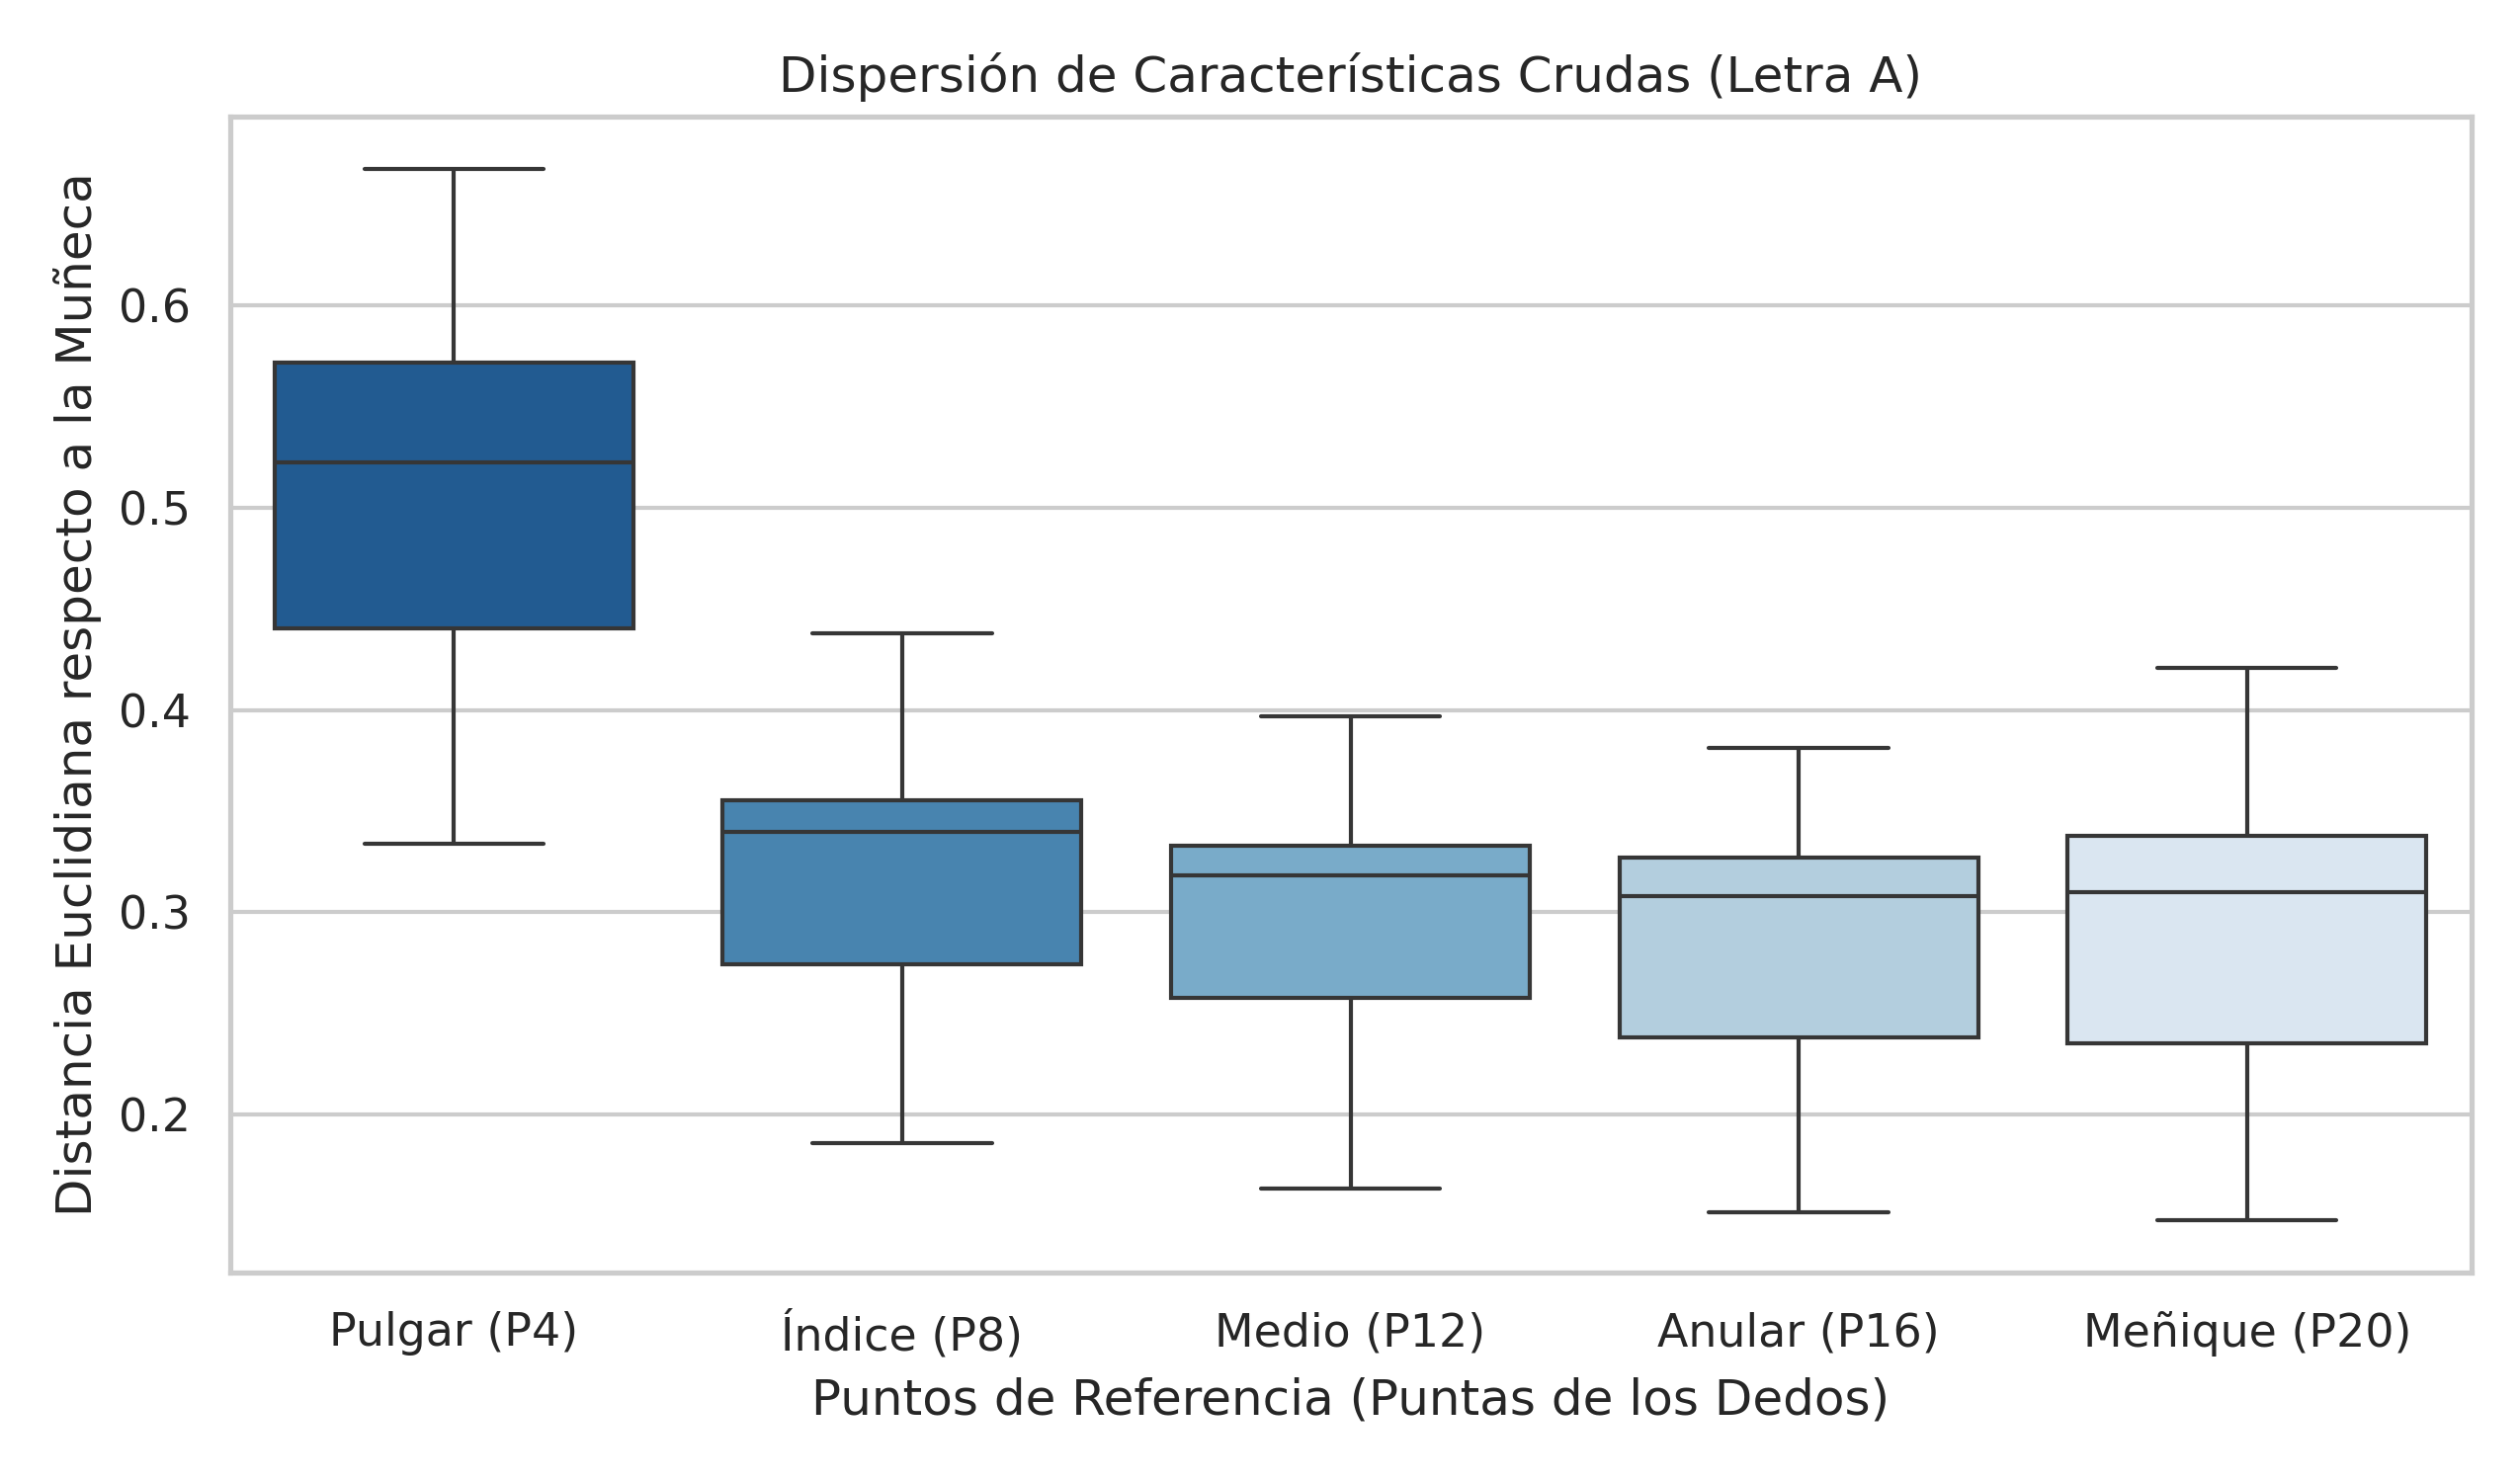
\includegraphics[width=0.85\textwidth]{images/nuevo_boxplot_letra_a.png}
		\caption{Dispersión de características crudas para la clase A}
		\label{fig:boxplot_variabilidad}
	\end{figure}
	Al analizar la Figura \ref{fig:boxplot_variabilidad}, se observa que todas las características presentan cajas amplias y bigotes extensos. El pulgar (\textit{landmark} 4), a pesar de mantener una postura fija y estirada en la seña A, muestra la caja más grande del gráfico debido a que la distancia absoluta medida en la pantalla cambia constantemente según la cercanía del usuario. Los dedos medio, anular y meñique exhiben rangos de distribución similares en la parte inferior debido a la flexión del puño. Este comportamiento confirma que las distancias absolutas en la pantalla arrastran toda la variabilidad del tamaño y encuadre de la captura, lo que reafirma la necesidad de aplicar una normalización propia centrada en la estructura interna de la mano.
	
	Para evaluar el impacto de esta variabilidad en escenarios de alta similitud morfológica, se realiza una comparación entre las señas más complejas del conjunto de datos: M, N, T, S, R y U. La Figura \ref{fig:boxplot_conflictivas} muestra la dispersión de la distancia calculada desde la muñeca hasta la punta del dedo índice (\textit{landmark} 8) para estas seis clases en su estado crudo.
	
	\begin{figure}[H]
		\centering
		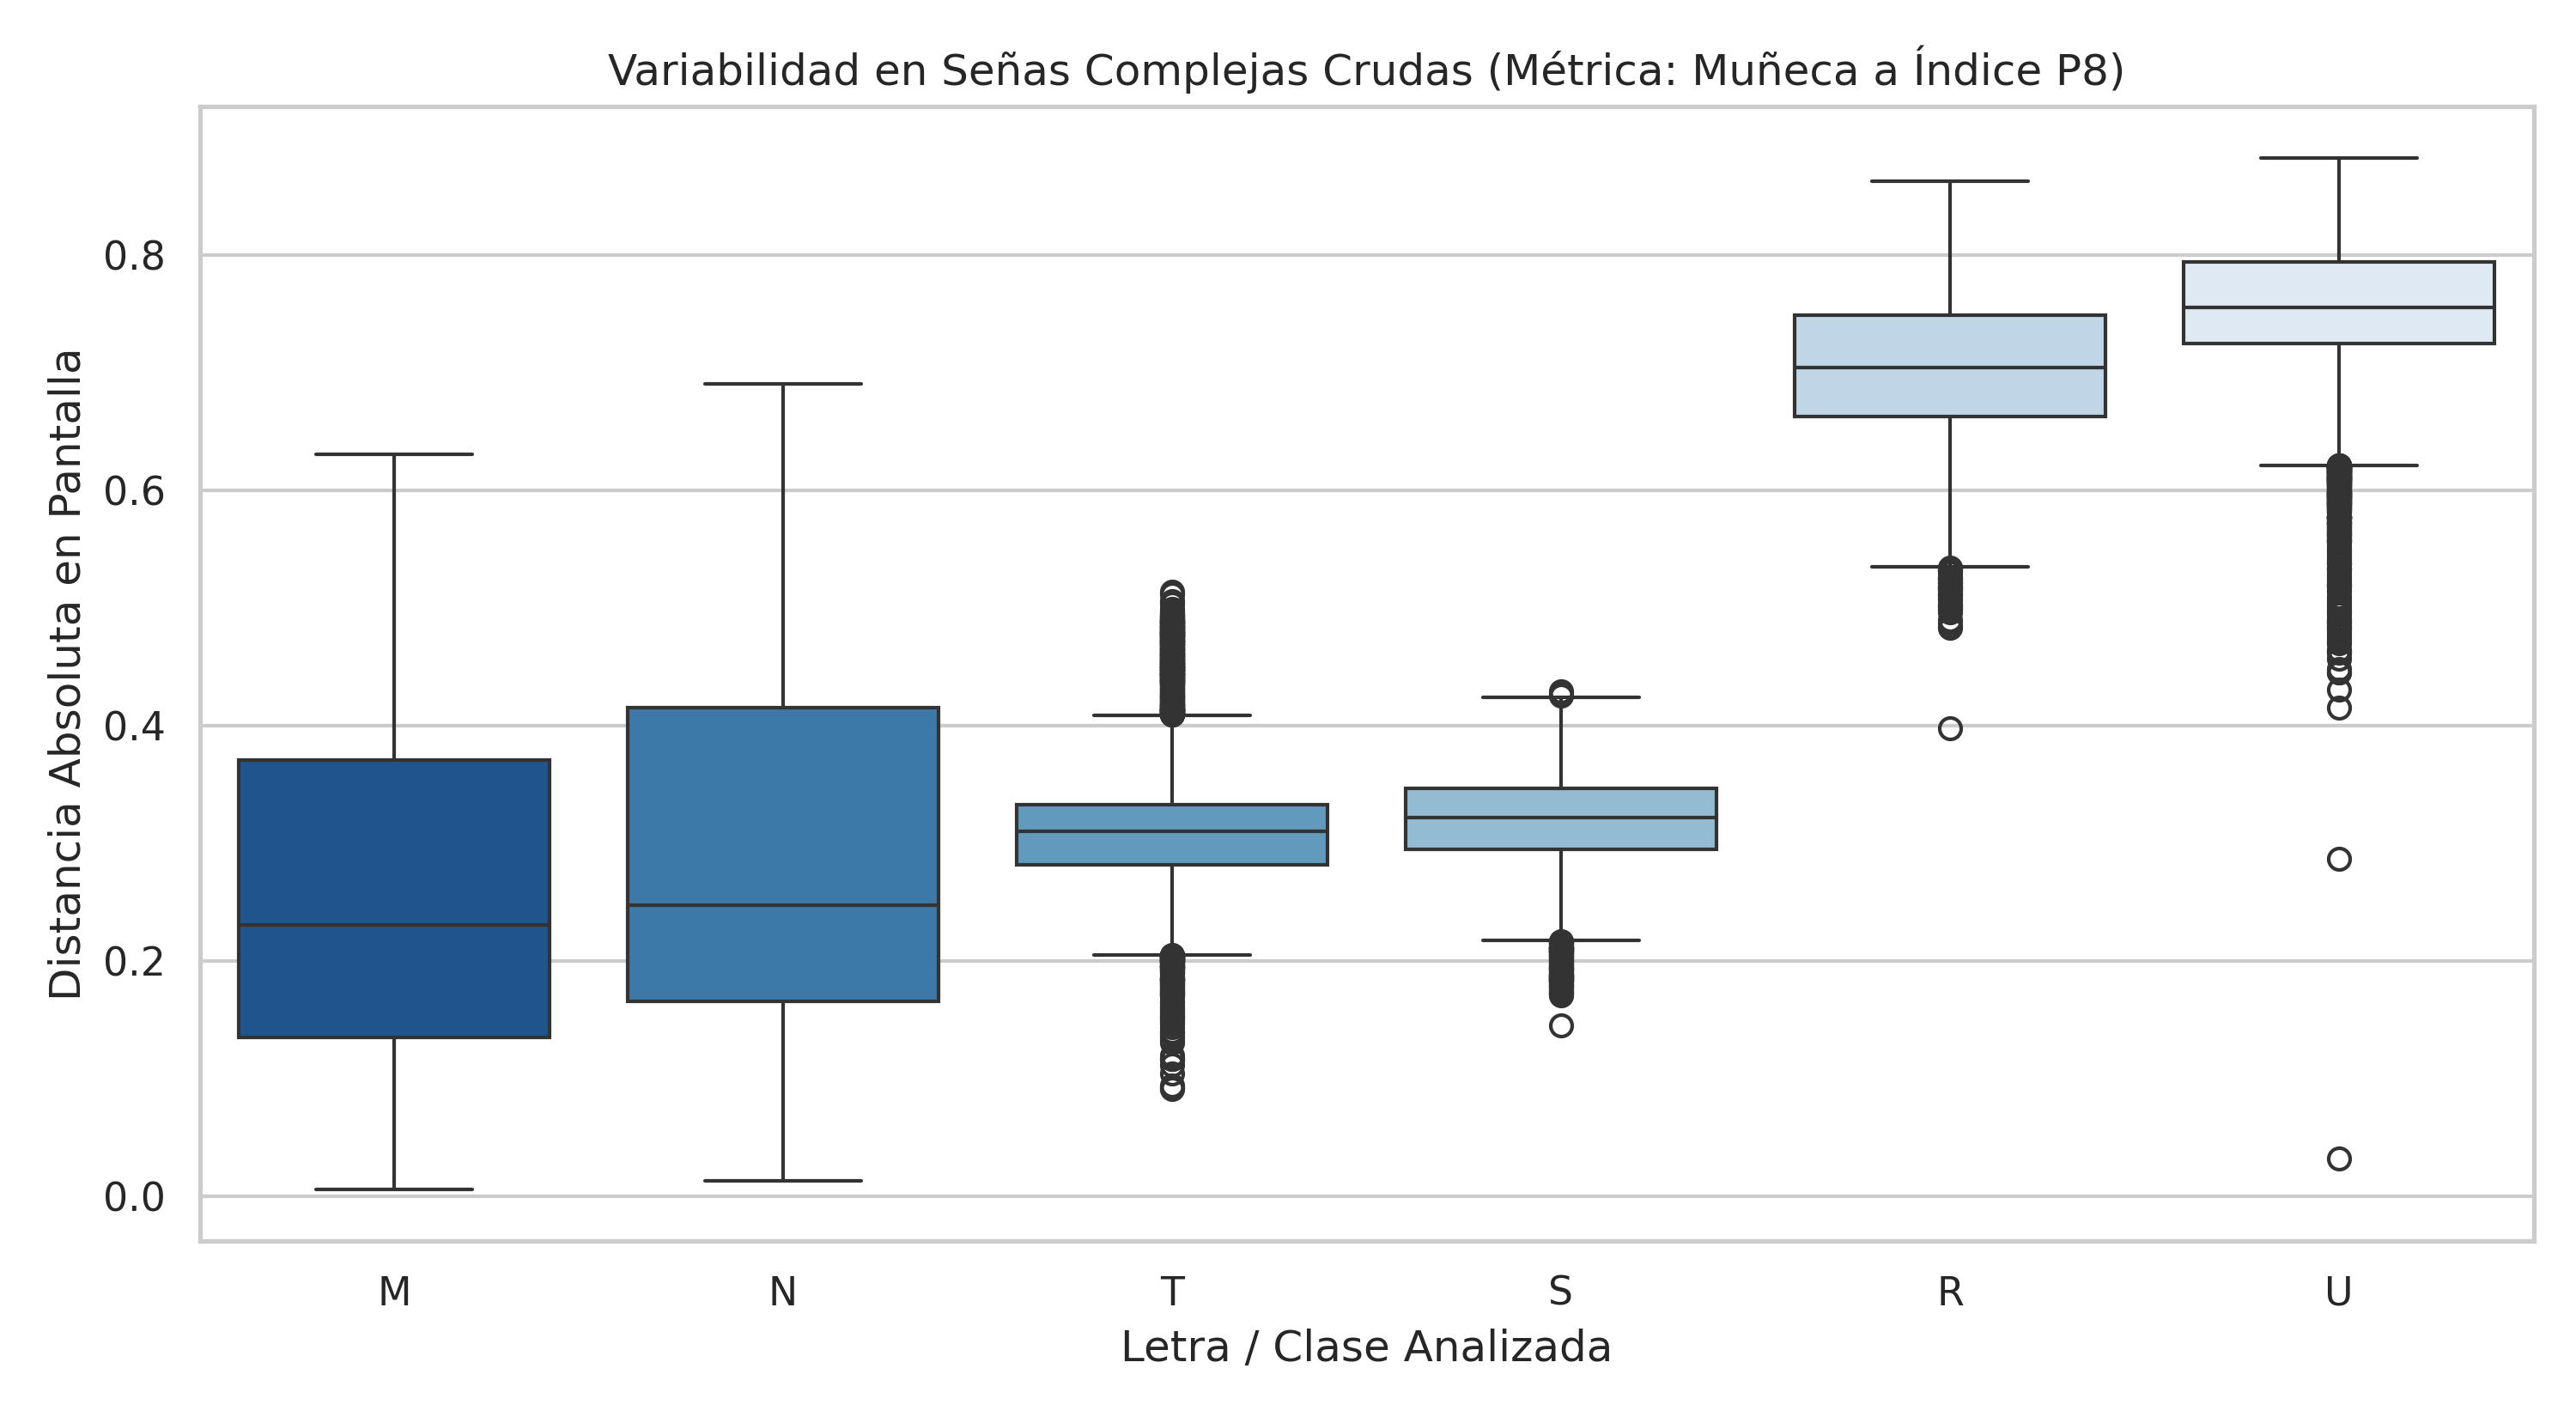
\includegraphics[width=0.85\textwidth]{images/nuevo_boxplot_conflictivas.png}
		\caption{Variabilidad en señas complejas crudas (Métrica: Muñeca a Índice P8)}
		\label{fig:boxplot_conflictivas}
	\end{figure}
	
	Los resultados de la Figura \ref{fig:boxplot_conflictivas} revelan problemas críticos para la clasificación sin un procesamiento previo:
	\begin{itemize}
		\item \textbf{Solapamiento por escala en letras cerradas (M y N):} Las letras M y N comparten casi el mismo nivel de distribución y tienen cajas muy anchas. Al depender del encuadre de la pantalla, una letra M capturada de cerca genera valores muy parecidos a una letra N capturada desde lejos, haciendo que los datos de cierta manera se encimen.
		\item \textbf{Ruido por oclusión y flexión (T y S):} Las señas T y S presentan cajas más compactas en la parte baja de la escala debido a que el índice va doblado. Sin embargo, la T muestra una enorme cantidad de puntos atípicos (\textit{outliers}) arriba y abajo, mientras que la S concentra sus errores principalmente en la parte inferior. Esto demuestra la inestabilidad que genera MediaPipe cuando el índice es obstruido por otros dedos al cerrar el puño.
		\item \textbf{Similitud de postura en letras abiertas (R y U):} Las cajas de las letras R y U se encuentran posicionadas en niveles altos y muy cercanos debido a que ambas mantienen el índice extendido. Aunque la U se encuentra ligeramente más arriba y compacta, la falta de una separación clara entre sus distribuciones provocaría errores de confusión masivos en el clasificador.
	\end{itemize}
	
	A partir de los resultados obtenidos en estas gráficas de variabilidad, queda clara la necesidad de buscar una forma de normalizar los datos para reducir el impacto de la distancia, el tamaño y la posición de los puntos. En esta etapa del proyecto, el interés principal no es saber en qué parte de la pantalla está la mano, ni qué tan lejos se encuentra el usuario o de qué tamaño es su extremidad. El objetivo real es conocer la forma exacta de la mano para poder clasificar cada seña de manera correcta.
	
	Por lo tanto los resultados de este análisis muestran que es necesario probar diferentes métodos de normalización. Esta revisión ayudará a encontrar la estrategia más estable para transformar los datos iniciales. En el desarrollo posterior se deberán hacer pruebas con distintas técnicas de centrado de puntos y cambios de escala, buscando la opción que mantenga la forma real de las señas de la LSM y reduzca el ruido provocado por los dedos ocultos.
	
	
	\subsubsection{Visualización del espacio de características mediante reducción dimensional}
	
	Cada muestra del conjunto de datos contiene un total de 42 dimensiones, las cuales corresponden a los ejes de las coordenadas de los puntos de la mano. Debido a que la percepción humana no puede interpretar un espacio con tantas dimensiones, resulta imposible evaluar de forma directa cómo se acomodan o se separan las diferentes clases a simple vista \cite{vandermaaten2008visualizing}. Por esta razón, es necesario realizar pruebas basadas en algoritmos de reducción de dimensiones para proyectar estos datos en una gráfica simple de dos dimensiones.
	
	En esta etapa del proyecto, esta técnica se utiliza como una herramienta de diagnóstico para revisar qué tan mezcladas o encimadas (\textit{overlapping}) quedan las señas antes de pasar al entrenamiento \cite{scikit-learn}. Ver la distribución visual de las letras permitirá entender la complejidad real del conjunto de datos crudos. Si las clases forman grupos separados y claros, se podría proponer el uso de clasificadores sencillos; por el contrario, si los datos quedan muy entrelazados debido al parecido físico de las señas, esto servirá como argumento sólido para justificar el uso de modelos más avanzados basados en redes neuronales \cite{geron2022hands}.
	
	
	\subsubsection{Visualización del espacio de características mediante reducción dimensional}
	
	Cada muestra del conjunto de datos contiene un total de 42 dimensiones, las cuales corresponden a los ejes de las coordenadas de los puntos de la mano. Debido a que la percepción humana no puede interpretar un espacio con tantas dimensiones, resulta imposible evaluar de forma directa cómo se acomodan o se separan las diferentes clases a simple vista \cite{vandermaaten2008visualizing}. Por esta razón, se utiliza el algoritmo de reducción de dimensiones t-SNE como una herramienta de diagnóstico visual en dos escenarios: con los datos crudos y con el dataset final preprocesado \cite{scikit-learn}.
	
	En primer lugar, se proyectó el universo de datos en su estado crudo, el cual incluye las variaciones absolutas de la pantalla. Los resultados de esta primera prueba se muestran en la Figura \ref{fig:tsne_completo}.
	
	\begin{figure}[H]
		\centering
		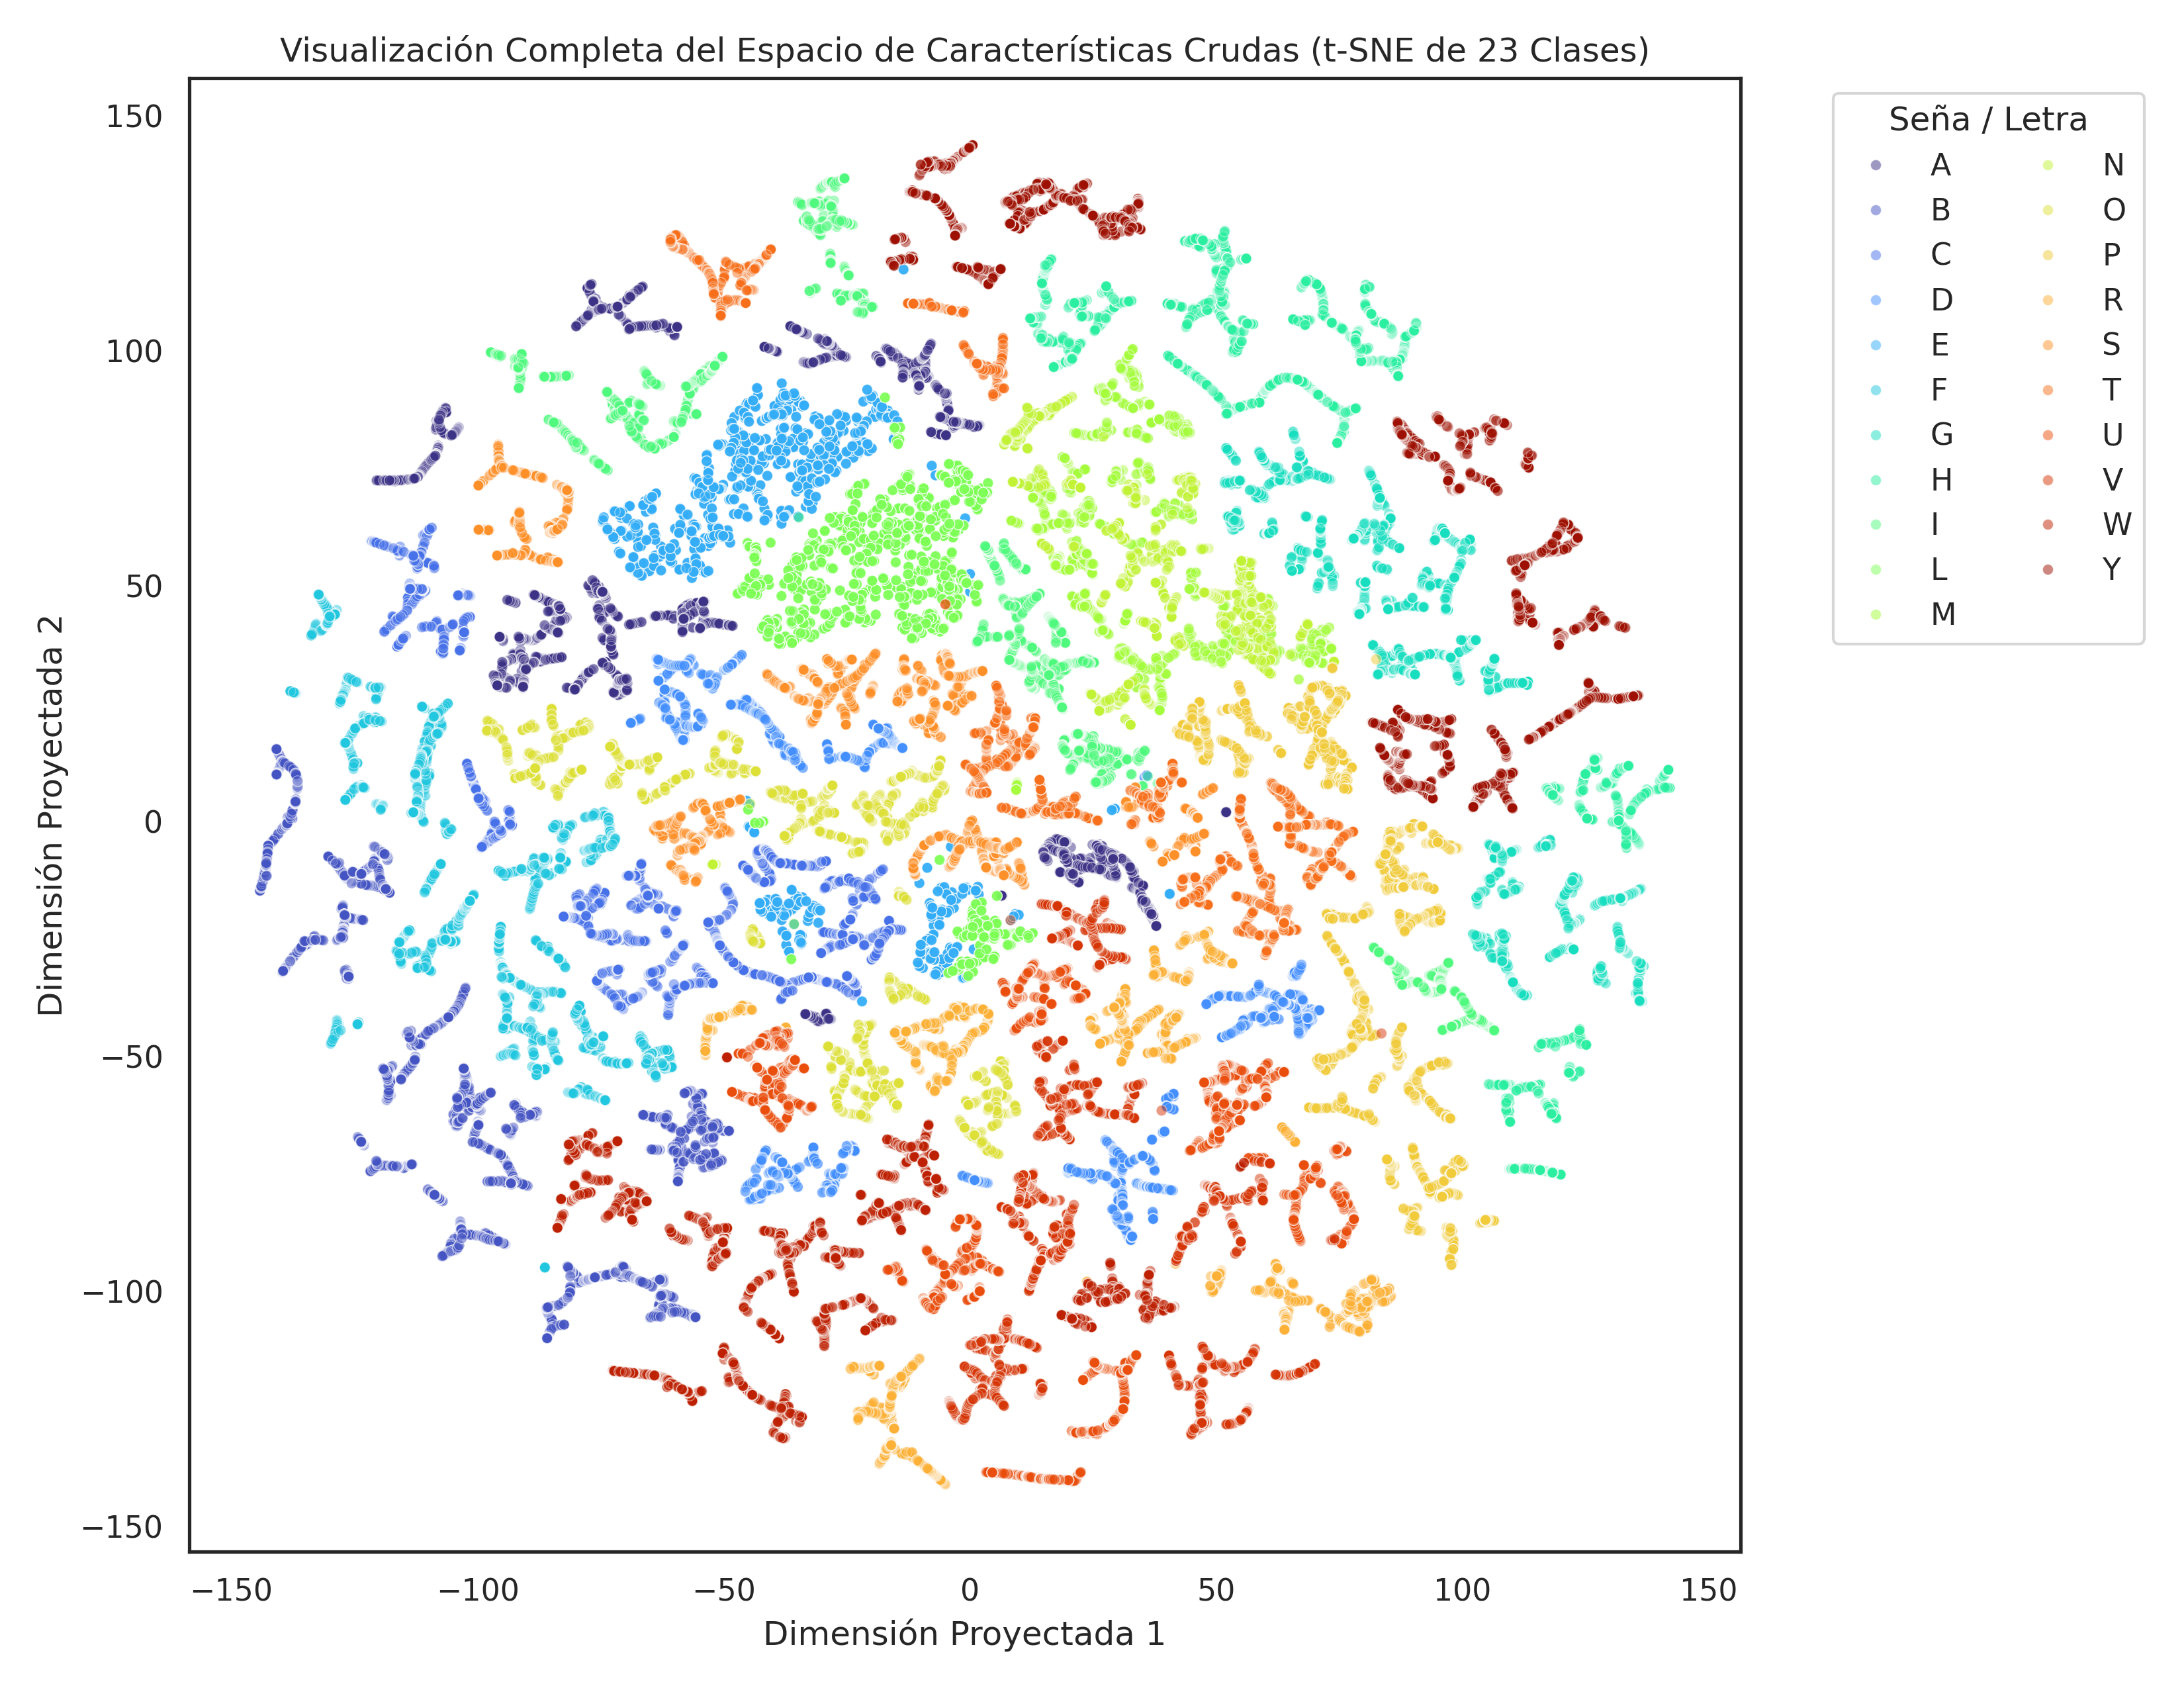
\includegraphics[width=0.85\textwidth]{images/tsne_dataset_completo.png}
		\caption{Visualización del espacio de características crudas mediante t-SNE}
		\label{fig:tsne_completo}
	\end{figure}
	
	Al analizar la estructura de la Figura \ref{fig:tsne_completo}, se observa una masa central amorfa donde clases como M, N, O, S y T se encuentran entrelazadas en algunas zonas. Asimismo, señas como B, C, L, W y Y se extienden hacia las orillas en forma de ramificaciones alargas. Este comportamiento confirma que los datos crudos arrastran toda la variabilidad de la distancia y el encuadre de la cámara, diluyendo las fronteras reales entre las letras de la LSM.
	
	Para comprobar la efectividad de las etapas de limpieza, se volvió a ejecutar el mismo algoritmo utilizando el dataset de 150000 muestras totalmente normalizado y preprocesado, listo para la etapa de entrenamiento. El resultado de esta proyección se observa en la Figura \ref{fig:tsne_normalizado}.
	
	\begin{figure}[H]
		\centering
		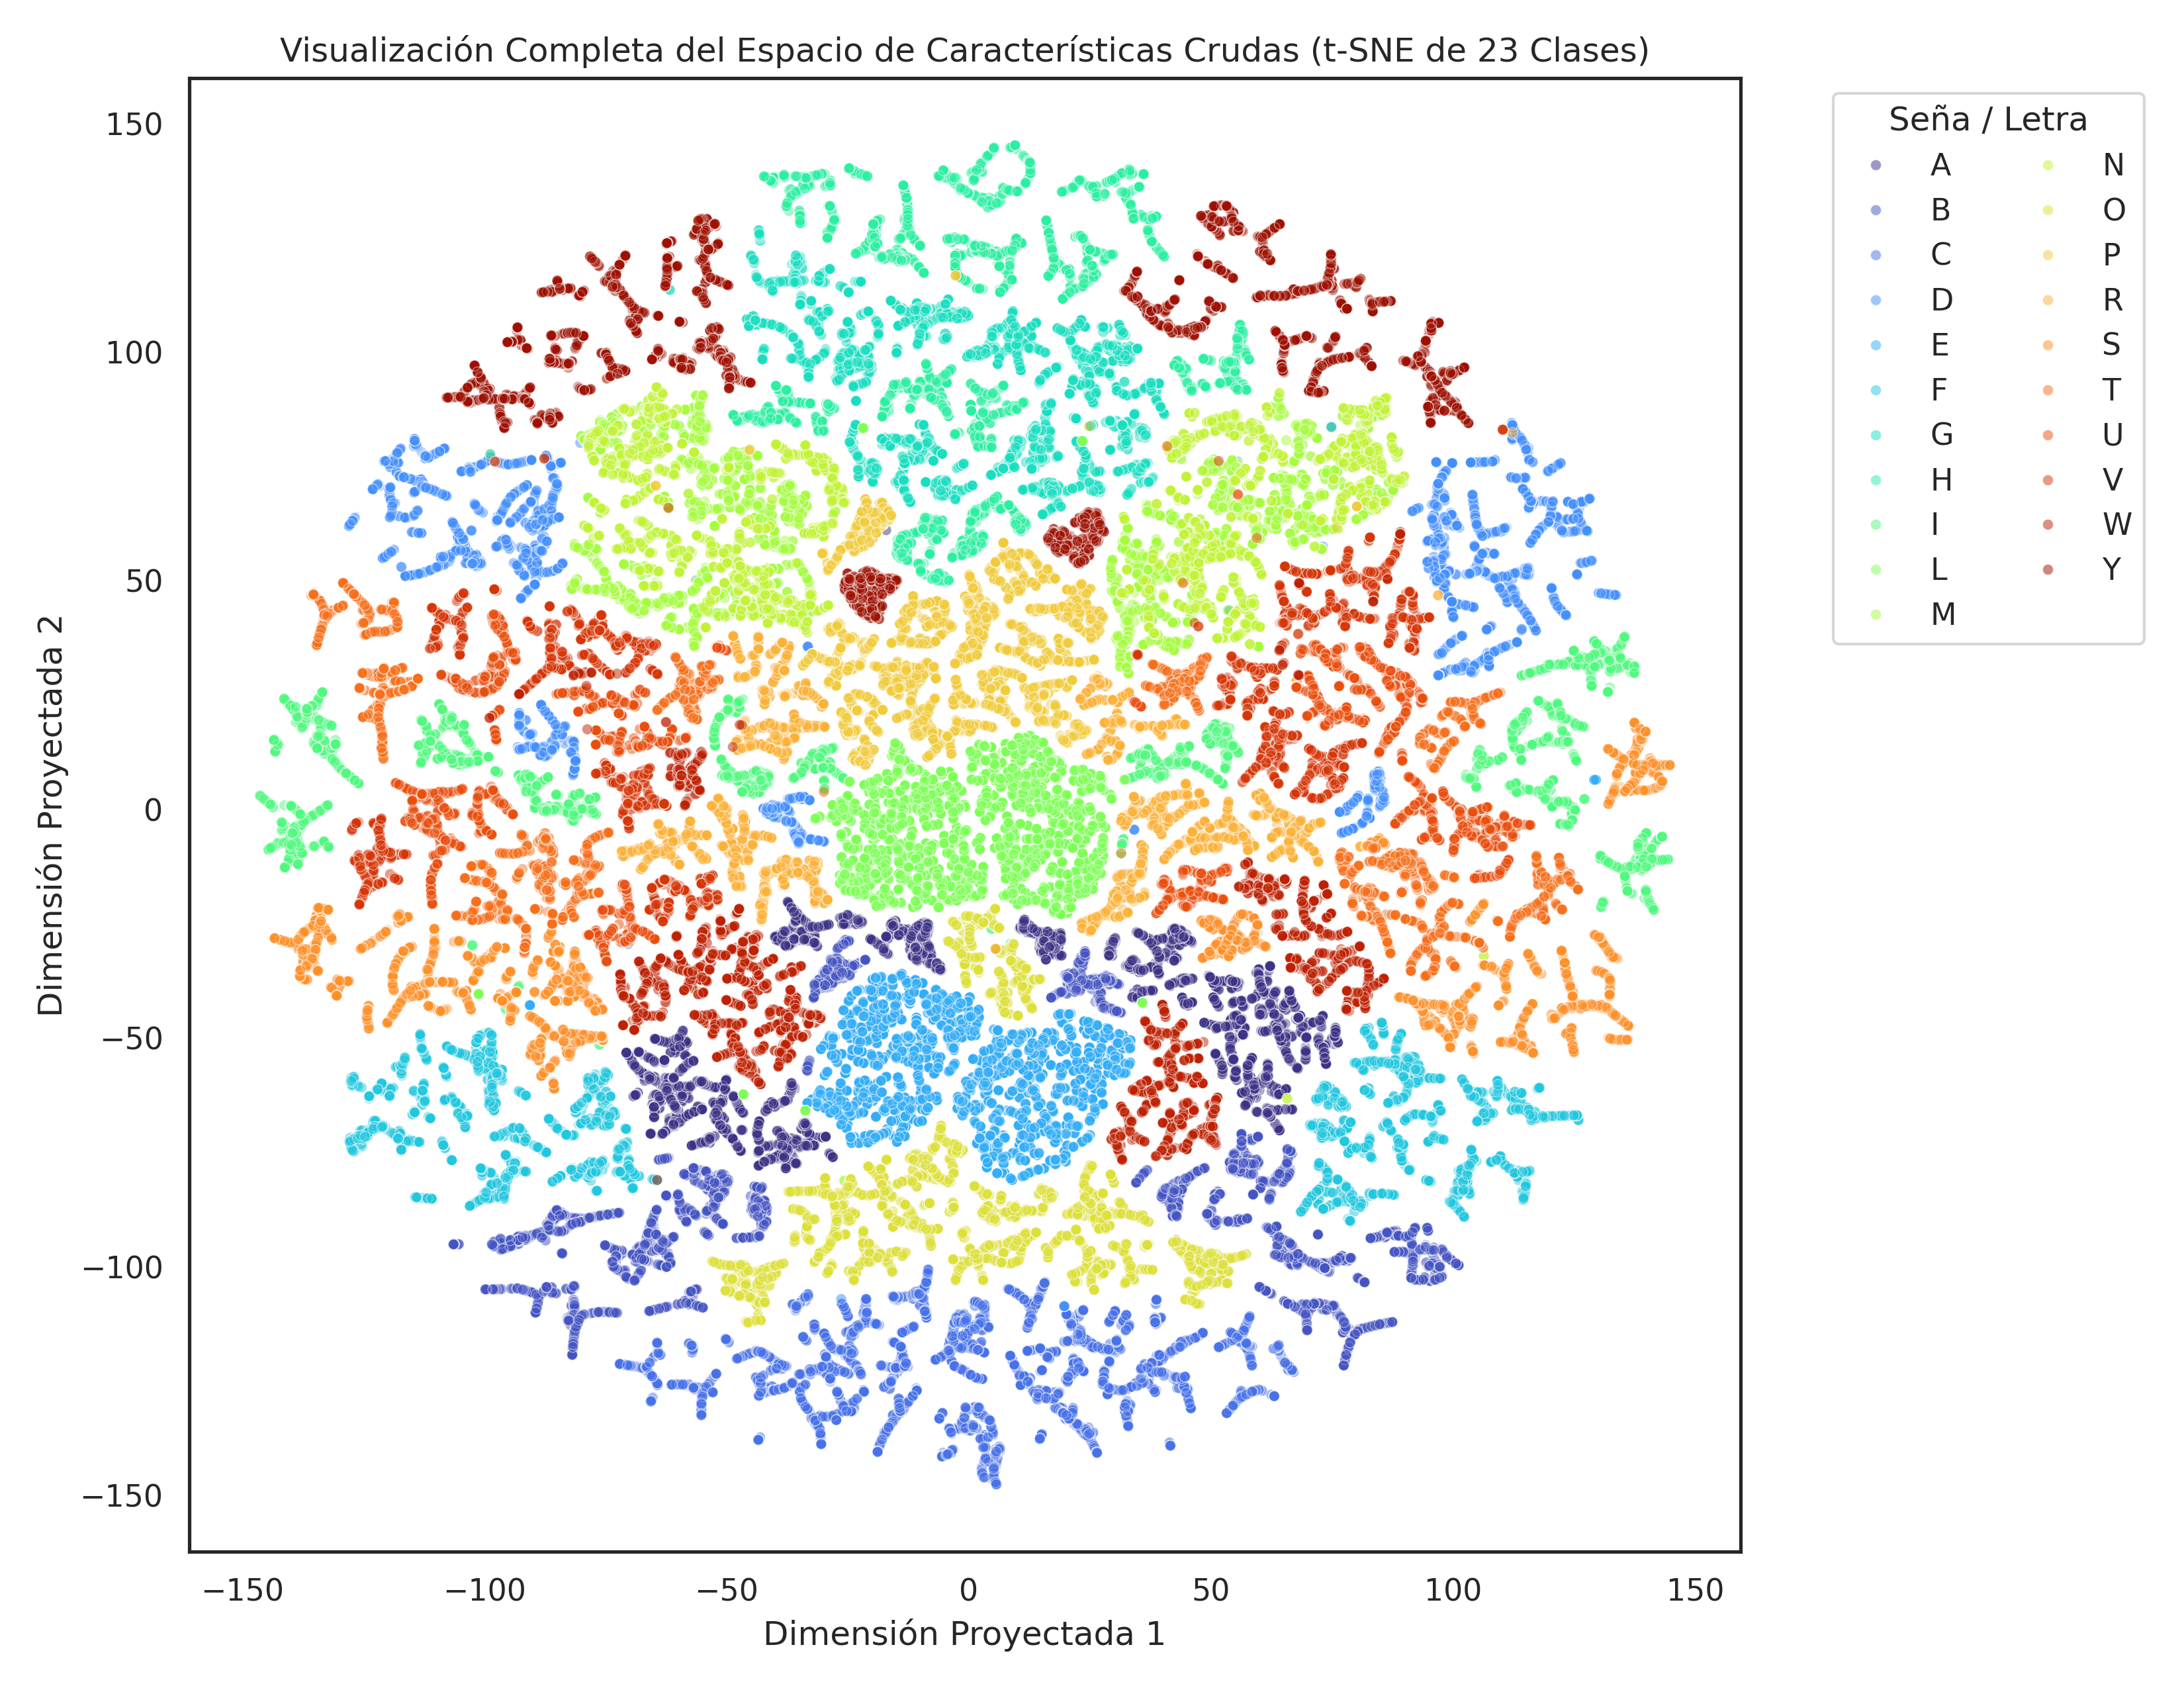
\includegraphics[width=0.85\textwidth]{images/tsne_dataset_completo_normalizadas.png}
		\caption{Visualización del espacio de características normalizadas listo para entrenamiento}
		\label{fig:tsne_normalizado}
	\end{figure}
	
	Al comparar la Figura \ref{fig:tsne_normalizado} con la proyección cruda anterior, se identifican cambios metodológicos fundamentales:
	\begin{itemize}
		\item \textbf{Compactación de clusters:} Las ramificaciones alargadas redujeron considerablemente. Al eliminar el factor de escala provocado por la distancia del usuario a la cámara, las muestras de una misma configuración geométrica se agruparon de forma densa y ordenada.
		\item \textbf{Estructura geométrica definida:} Los datos se reacomodaron en agrupaciones mas grandes y continuas que reflejan la transición física real entre las posturas de los dedos.
		\item \textbf{Complejidad no lineal persistente:} A pesar de la notable limpieza y orden en los datos, las clases siguen compartiendo fronteras sumamente complejas. En la región central y en las zonas periféricas se aprecia cómo clusters de diferentes colores se rodean y colindan directamente entre sí sin llegar a separarse de forma aislada.
	\end{itemize}
	
	La distribución visual obtenida en el escenario preprocesado demuestra  que el problema de reconocimiento de la LSM no es linealmente separable. Intentar resolver este sistema mediante clasificadores estadísticos simples o modelos lineales provocaría un porcentaje de error en la aplicación móvil, ya que estos algoritmos son incapaces de trazar límites curvos y complejos en zonas de alta colindancia como las que exhiben algunas letras  letras.
	
	La comparación de ambos espacios de características justifica la selección tecnológica de este proyecto: el algoritmo de normalización local propuesto es indispensable para ordenar el espacio numérico, mientras que el uso de una arquitectura basada en redes neuronales artificiales será la mejor opción, ya que es la única herramienta capaz de aprender fronteras no lineales de alta complejidad para asegurar una clasificación robusta y precisa en el dispositivo final \cite{geron2022hands}.
	
	\subsection{Conclusiones del análisis exploratorio}
	
	A partir del análisis exploratorio, se determina que el éxito del clasificador embebido en un dispositivo móvil no depende de buscar un modelo de aprendizaje profundo exageradamente grande o complejo. El verdadero rendimiento del sistema radica en encontrar una configuración de normalización adecuada combinada con un ajuste correcto de hiperparámetros para entrenar la red neuronal.
	
	Los datos crudos muestran problemas en su estructura que exigen realizar pruebas rigurosas. A continuación, se detallan los retos del entorno real y la ruta de trabajo justificada por las gráficas estadísticas anteriores.
	
	\subsubsection{Caminos para la experimentación y normalización de datos}
	
	Los resultados del histograma de escala y las proyecciones t-SNE demostraron que la normalización general mediante cajas delimitadoras (\textit{bounding boxes}) ayuda a que los datos no se salgan de la pantalla, pero no es suficiente. Este método deforma las proporciones de la mano cuando el usuario abre o cierra el puño. Por lo tanto, las siguientes pruebas deben enfocarse en quitar la dependencia de la pantalla y diseñar un forma de normalizar basado únicamente en la estructura de la mano, evaluando tres estrategias :
	
	\begin{itemize}
		\item \textbf{Uso de un punto de anclaje local:} En lugar de usar los extremos de la pantalla, las pruebas deben orientarse a usar un punto fijo de la mano como el centro del mapa de coordenadas. El punto ideal es la muñeca (\textit{landmark} 0) o la base del dedo medio (\textit{landmark} 9). Al restar la posición de este punto central a todos los demás, se calcula un vector de desplazamiento local que elimina el problema de si la mano se mueve de lugar en la pantalla.
		\item \textbf{Ajuste de escala por el tamaño de la palma:} Para solucionar los cambios de tamaño provocados por la distancia, se debe probar un factor de división basado en una distancia de la mano que casi nunca cambie, como la línea que va de la muñeca a la base del dedo medio ($||P_9 - P_0||$). Al dividir todas las coordenadas entre esta distancia, el tamaño de la mano se estandariza sin importar si el usuario está muy cerca o lejos de la cámara del celular.
		\item \textbf{Corrección por inclinación de la mano:} El análisis de los datos crudos asume que la mano siempre está derecha. En el uso real, la gente inclina la muñeca de forma natural. Es necesario experimentar con fórmulas de rotación geométrica basadas en el ángulo de la palma, buscando que los datos finales sean los mismos aunque el usuario gire un poco la mano o el celular.
	\end{itemize}
	
	\subsubsection{Retos del entorno real y problemas físicos}
	
	Llevar un traductor de señas a un teléfono móvil introduce variables del mundo físico que pueden alterar los números que recibe el sistema. Las gráficas de boxplot mostraron que MediaPipe mete ruido cuando se presentan ciertas condiciones, las cuales representan los principales retos de ingeniería para el proyecto:
	
	\begin{itemize}
		\item \textbf{Dedos ocultos o tapados entre sí:} Este es el reto más difícil en las señas que llevan el puño cerrado o los dedos cruzados como M, N, T y S. Cuando un dedo tapa a otro frente a la cámara, el sistema de MediaPipe pierde la vista directa y empieza a calcular la posición del punto oculto mediante estimaciones. Esto genera datos erróneos y saltos bruscos en las coordenadas (los puntos atípicos u \textit{outliers} que vimos en las gráficas). Las pruebas con el modelo deben ser capaces de absorber este ruido para evitar fallas en la aplicación.
		\item \textbf{Señas que se parecen físicamente:} El t-SNE del dataset normalizado dejó claro que letras como R y U, o M y N, se quedan pegadas en el mapa porque la postura de la mano es casi la misma. El enfoque de los experimentos no debe ser solo separar grupos grandes, sino lograr que el sistema detecte los detalles más pequeños, como la separación milimétrica entre las puntas de los dedos o el cruce exacto del pulgar. Si el procesamiento no resalta estas diferencias, el modelo final va a confundir estas letras constantemente.
		\item \textbf{Cambios de luz y ruido en la cámara:} Las cámaras de los celulares cambian su configuración dependiendo de la luz del cuarto. Cuando hay poca iluminación, la imagen pierde nitidez y los bordes de los dedos se ven borrosos, haciendo que los puntos de MediaPipe tiemblen de un cuadro a otro aunque la mano esté quieta. Este temblor en las coordenadas se debe controlar mediante filtros matemáticos antes de mandar los datos al clasificador.
		\item \textbf{Ángulo de la toma y perspectiva:} El usuario común no va a sostener el celular en una posición perfecta frente a su rostro. Si el teléfono se inclina, los dedos estirados se verán más cortos en la pantalla de lo que realmente son debido a la perspectiva. Para superar esto, las transformaciones matemáticas en el preprocesamiento deben aprovechar la coordenada de profundidad relativa que ofrece el sensor para corregir la postura en un entorno tridimensional virtual.
	\end{itemize}
	
	
	La evidencia que dejaron las gráficas cierra por completo la posibilidad de usar reglas fijas o algoritmos estadísticos simples. El mapa de las 21 letras, incluso estando normalizado y limpio, muestra que las fronteras entre las señas de la LSM no son líneas rectas, sino curvas y pliegues complejos donde unas clases rodean a otras, especialmente en el grupo de M, N, S y T.
	
	Los principales retos serán:
	
	1. Crear un proceso de limpieza de características propio y local que unifique el tamaño y rotación de la mano, eliminando el ruido de la pantalla antes de que los datos lleguen al clasificador.
	2. Implementar un MLP entrenado específicamente para aprender estas fronteras curvas y complejas que los modelos lineales sencillos no pueden resolver.
	
	Esta combinación asegura que las pequeñas diferencias entre las señas difíciles puedan separarse con alta precisión, consumiendo muy pocos recursos del teléfono al exportar el modelo final en formato TensorFlow Lite.
	
	
	\subsection{Consideraciones de uso y privacidad}
	
	VisionLSM es un prototipo académico y experimental desarrollado como parte de un trabajo terminal del Instituto Politécnico Nacional, cuyo objetivo principal consiste en desarrollar un prototipo para reconocimiento de señas estáticas de la LSM en dispositivos móviles Android mediante visión por computadora.
	
	Debido a la naturaleza experimental del proyecto, la aplicación se encuentra en una etapa de desarrollo y validación, por lo que su funcionamiento puede presentar variaciones dependiendo de las condiciones de uso, el dispositivo empleado y el entorno de captura. El sistema fue diseñado con fines académicos, de investigación y demostración tecnológica, por lo que no debe considerarse un producto comercial ni un sistema definitivo para comunicación asistida.
	
	Actualmente la aplicación no se encuentra distribuida mediante Google Play Store debido a que se trata de un prototipo en fase de evaluación académica. Es por eso que la instalación de la aplicación debe realizarse manualmente mediante un archivo .apk proporcionado por los desarrolladores o responsables del proyecto.
	
	El usuario reconoce y acepta que la instalación de aplicaciones externas mediante archivos .apk puede requerir la habilitación de permisos especiales dentro del sistema operativo Android, así como la aceptación de configuraciones relacionadas con la instalación de aplicaciones provenientes de fuentes externas a Google Play Store.
	
	Asimismo, el usuario acepta que el uso de la aplicación se realiza bajo su propia responsabilidad. Los desarrolladores no garantizan un funcionamiento libre de errores ni una precisión absoluta en las inferencias realizadas por el sistema, debido a las limitaciones inherentes a los modelos de inteligencia artificial y a las condiciones variables presentes durante el reconocimiento de señas. De igual forma el prototipo no sustituye la labor de intérpretes profesionales y certificados de LSM ni debe considerarse un sistema oficial de traducción o asistencia para la comunicación.
	
	El uso del prototipo implica la aceptación de las consideraciones técnicas, limitaciones operativas y condiciones descritas en el presente documento.

	

	\subsection{Términos y condiciones de uso}
	
	\subsubsection{Aceptación de los términos}
	
	El uso, instalación o acceso a la aplicación VisionLSM implica que el usuario ha leído, comprendido y aceptado los presentes términos y condiciones de uso, así como las disposiciones descritas en el aviso de privacidad incluido en el presente documento.
	
	En caso de que el usuario no esté de acuerdo con alguna de las condiciones establecidas, deberá abstenerse de instalar o utilizar la aplicación.
	
	Asimismo, el usuario reconoce que la aplicación corresponde a un prototipo académico y experimental, por lo que acepta las limitaciones técnicas, operativas y funcionales propias del sistema, así como el uso de la aplicación bajo su propia responsabilidad.
	
	\subsubsection{Uso permitido}
	
	El usuario se compromete a utilizar la aplicación únicamente con fines lícitos, éticos y compatibles con los objetivos académicos y tecnológicos del proyecto.
	
	Se permite el uso de la aplicación para:
	
	\begin{itemize}
		\item Actividades académicas y educativas.
		
		\item Pruebas experimentales relacionadas con el reconocimiento de señas.
		
		\item Evaluación y demostración del funcionamiento del prototipo.
		
		\item Actividades de investigación orientadas al análisis de modelos de inteligencia artificial y visión por computadora.
		
		\item Apoyo experimental a procesos de comunicación mediante reconocimiento de señas.
	\end{itemize}
	
	El uso de la aplicación deberá realizarse respetando en todo momento la privacidad, integridad y derechos de terceros.
	
	\subsubsection{Restricciones de uso}
	
	Queda prohibido utilizar la aplicación para actividades contrarias a la ley, la ética o los objetivos académicos para los cuales fue desarrollada.
	
	El usuario se compromete a no:
	
	\begin{itemize}
		\item Modificar, descompilar, alterar o intentar vulnerar el funcionamiento interno de la aplicación sin autorización de los desarrolladores.
		
		\item Utilizar el sistema con fines ilícitos, fraudulentos o que puedan afectar a terceros.
		
		\item Emplear la aplicación para actividades discriminatorias, ofensivas o que vulneren derechos humanos.
		
		\item Utilizar la aplicación como sustituto de servicios profesionales, intérpretes certificados o mecanismos oficiales de comunicación.
		
		\item Intentar acceder, manipular o alterar componentes internos relacionados con el modelo de inteligencia artificial, procesamiento de imágenes o funcionamiento del sistema.
		
		\item Distribuir versiones modificadas de la aplicación sin autorización expresa de los desarrolladores.
	\end{itemize}
	
	Cualquier uso indebido de la aplicación será responsabilidad exclusiva del usuario.
	
	\subsubsection{Limitaciones del sistema}
	
	El usuario reconoce que VisionLSM corresponde a un prototipo experimental basado en modelos de inteligencia artificial y visión por computadora, por lo que el sistema puede presentar errores, variaciones o limitaciones durante el reconocimiento de señas.
	
	La precisión del reconocimiento puede verse afectada por diferentes factores, entre ellos:
	
	\begin{itemize}
		\item Condiciones de iluminación insuficientes o excesivas.
		
		\item Fondos visualmente complejos o con múltiples objetos.
		
		\item Oclusiones parciales o total de la mano.
		
		\item Posicionamiento incorrecto respecto a la cámara.
		
		\item Distancias inadecuadas entre la mano y el dispositivo móvil.
		
		\item Movimientos rápidos o inestables durante la captura.
		
		\item Variaciones físicas entre usuarios, tales como tamaño de mano, orientación o forma de realizar las señas.
		
		\item Limitaciones inherentes al modelo de inteligencia artificial utilizado.
	\end{itemize}
	
	Con base en lo anterior los resultados generados por la aplicación deben considerarse de carácter orientativo y experimental, por lo que no se garantiza una precisión absoluta en todas las condiciones de uso.
	
	El sistema no sustituye intérpretes profesionales de Lengua de Señas Mexicana ni debe utilizarse como herramienta oficial de traducción o asistencia crítica para la comunicación.
	
	\subsubsection{Disponibilidad del servicio}
	
	Dado que VisionLSM corresponde a un prototipo académico y experimental en fase de desarrollo y evaluación tecnológica, no se garantiza la disponibilidad permanente del sistema ni el funcionamiento ininterrumpido de la aplicación en todos los dispositivos móviles Android.
	
	La compatibilidad del sistema puede variar dependiendo de factores como:
	
	\begin{itemize}
		\item Versión del sistema operativo Android.
		
		\item Capacidades de hardware del dispositivo.
		
		\item Calidad y resolución de la cámara.
		
		\item Recursos disponibles del sistema, tales como memoria RAM y capacidad de procesamiento.
		
		\item Configuraciones internas del dispositivo móvil.
	\end{itemize}
	
	Asimismo, los desarrolladores podrán suspender temporalmente el funcionamiento del sistema, realizar modificaciones o actualizar componentes de la aplicación con fines académicos, de mantenimiento, corrección de errores o mejora del prototipo.
	
	Debido a la naturaleza experimental del proyecto, no se garantiza compatibilidad absoluta, disponibilidad continua ni estabilidad total en todas las condiciones de uso.
	
	\subsubsection{Responsabilidad del usuario}
	
	El usuario es responsable del uso que realice de la aplicación, así como de la instalación del archivo .apk en su dispositivo móvil y de la configuración de los permisos necesarios para el funcionamiento del sistema.
	
	Antes de utilizar la aplicación, el usuario deberá otorgar permiso explícito para el acceso a la cámara del dispositivo, reconociendo que dicho recurso es indispensable para el funcionamiento del sistema de reconocimiento de señas.
	
	El usuario también acepta utilizar la aplicación en entornos adecuados y seguros, respetando en todo momento la privacidad, integridad y derechos de terceros. Los desarrolladores no se hacen responsables por el uso indebido de la aplicación, ni por posibles afectaciones derivadas de configuraciones incorrectas, incompatibilidades del dispositivo o interpretaciones erróneas generadas por el sistema.
	
	Debido a que la instalación se realiza mediante un archivo .apk externo y no a través de Google Play Store, el usuario reconoce y acepta los riesgos asociados a la instalación manual de aplicaciones provenientes de fuentes externas, así como la responsabilidad derivada de habilitar los permisos correspondientes dentro del sistema operativo Android.
	
	\subsubsection{Propiedad intelectual}
	
	El código fuente, arquitectura de software, modelos de inteligencia artificial, documentación, diseño de interfaces y demás componentes desarrollados para VisionLSM forman parte del trabajo terminal realizado en el Instituto Politécnico Nacional con fines académicos y de investigación tecnológica.
	
	Todos los elementos desarrollados dentro del proyecto se encuentran protegidos por las disposiciones aplicables en materia de propiedad intelectual y derechos de autor. La reproducción, distribución, modificación o utilización total o parcial del sistema con fines comerciales requerirá autorización expresa de los autores del proyecto.
	
	El uso académico y demostrativo de la aplicación no otorga al usuario derechos de propiedad sobre el software, los modelos de inteligencia artificial, la documentación técnica ni sobre cualquier componente relacionado con el desarrollo del prototipo.
	
	Las bibliotecas, frameworks y herramientas de terceros utilizadas durante el desarrollo del sistema conservan los derechos y licencias establecidos por sus respectivos propietarios y desarrolladores.
	
	\subsection{Aviso de privacidad}

	\subsubsection{Información recopilada}
	
	Para el funcionamiento de VisionLSM, la aplicación puede acceder a determinados recursos y datos básicos del dispositivo móvil, necesarios para ejecutar el sistema de reconocimiento de señas.
	
	La aplicación solicita acceso a:
	
	\begin{itemize}
		\item Cámara del dispositivo móvil.
		
		\item Información básica relacionada con el funcionamiento del sistema operativo y capacidades generales del dispositivo.
	\end{itemize}
	
	El acceso a la cámara es indispensable para capturar temporalmente imágenes durante el proceso de detección y reconocimiento de señas realizadas por el usuario.
	
	Cierta información técnica del dispositivo puede ser utilizada de manera limitada con fines relacionados con compatibilidad, ejecución del sistema y funcionamiento general de la aplicación. En ningún caso esta información es utilizada con fines comerciales, publicitarios o de rastreo del usuario.
	
	\subsubsection{Datos procesados}
	
	Durante el funcionamiento de VisionLSM, el sistema realiza el procesamiento temporal de información necesaria para ejecutar el reconocimiento y clasificación de señas.
	
	Los datos procesados por la aplicación pueden incluir:
	
	\begin{itemize}
		\item Imágenes capturadas temporalmente por la cámara del dispositivo móvil durante el reconocimiento.
		
		\item Coordenadas y puntos de referencia de la mano obtenidos mediante algoritmos de detección y seguimiento.
		
		\item Resultados generados por el modelo de inteligencia artificial, tales como letras o señas reconocidas y niveles de confianza asociados a la inferencia.
	\end{itemize}
	
	La información procesada es utilizada exclusivamente para ejecutar las funciones de reconocimiento de señas, evaluación del desempeño del sistema y funcionamiento general del prototipo.
	
	El procesamiento de esta información se realiza de manera temporal y únicamente durante la interacción activa del usuario con la aplicación.
	
	\subsubsection{Datos no recopilados}
	
	VisionLSM no recopila, almacena ni comparte de manera permanente información personal sensible del usuario durante el funcionamiento normal de la aplicación.
	
	La aplicación no solicita ni procesa:
	
	\begin{itemize}
		\item Información bancaria o financiera.
		
		\item Contraseñas o credenciales de acceso.
		
		\item Ubicación geográfica mediante GPS.
		
		\item Información de contactos personales.
		
		\item Mensajes privados o contenido externo al funcionamiento de la aplicación.
		
		\item Fotografías o videos almacenados permanentemente en el dispositivo.
		
		\item Datos biométricos persistentes orientados a identificación personal.
	\end{itemize}
	
	Las imágenes capturadas temporalmente durante el reconocimiento de señas no son almacenadas de manera permanente durante el uso normal del sistema.
	
	\subsubsection{Procesamiento local}
	
	VisionLSM realiza el procesamiento principal de imágenes y la ejecución del modelo de inteligencia artificial directamente en el dispositivo móvil del usuario, mediante técnicas de inferencia local.
	
	Esto significa que las imágenes capturadas por la cámara y los datos generados durante el reconocimiento de señas son procesados principalmente dentro del propio dispositivo, reduciendo la necesidad de transferir información hacia servidores externos o servicios en la nube.
	
	El enfoque de procesamiento local permite:
	
	\begin{itemize}
		\item Disminuir la exposición de información visual del usuario.
		
		\item Reducir riesgos asociados a la transferencia de datos.
		
		\item Mejorar la privacidad durante el uso de la aplicación.
		
		\item Permitir el funcionamiento del sistema sin conexión permanente a internet.
	\end{itemize}
	
	Durante el funcionamiento normal de la aplicación, las inferencias realizadas por el modelo de clasificación no requieren el envío continuo de imágenes, videos o datos personales a plataformas externas para ejecutar el reconocimiento de señas.
	
	
	\subsubsection{Cumplimiento normativo}
	
	El tratamiento y procesamiento de la información dentro de VisionLSM se realiza considerando principios de privacidad, confidencialidad y minimización de datos establecidos en la legislación mexicana aplicable en materia de protección de datos personales, especificamente en la Ley Federal de Protección de Datos Personales en Posesión de los Particulares (LFPDPPP).
	
	Debido a la naturaleza académica y experimental del proyecto, los datos procesados por la aplicación son utilizados exclusivamente con fines relacionados con el funcionamiento del sistema.
	
	El diseño de la aplicación considera medidas orientadas a reducir la exposición innecesaria de información del usuario, priorizando el procesamiento local de imágenes, la minimización de datos procesados y la no recopilación permanente de información personal sensible durante el funcionamiento normal del sistema.

		
	\subsubsection{Aceptación del aviso de privacidad}
	
	El uso, instalación o acceso a la aplicación VisionLSM implica que el usuario ha leído, comprendido y aceptado las disposiciones establecidas en el presente aviso de privacidad.
	
	Asimismo, el usuario reconoce y acepta que la aplicación requiere acceso temporal a la cámara del dispositivo móvil para ejecutar las funciones de reconocimiento de señas descritas en el presente manual.
	
	En caso de que el usuario no esté de acuerdo con las condiciones relacionadas con el tratamiento y procesamiento de la información descritas en este documento, deberá abstenerse de instalar o utilizar la aplicación.
	
	El consentimiento otorgado por el usuario se limita exclusivamente al funcionamiento académico, experimental y tecnológico del prototipo desarrollado dentro del presente Trabajo Terminal.
	
	
	
